\documentclass[11pt,a4paper,notitlepage]{article}
\usepackage[margin=3cm]{geometry}
\usepackage{amsmath}
\usepackage{amsfonts}
\usepackage{graphicx}
\usepackage{color}
\usepackage[most]{tcolorbox}

\tcbset{colback=white!10!white, colframe=black!50!black, 
        highlight math style= {enhanced, %<-- needed for the ’remember’ options
            colframe=red,colback=red!10!white,boxsep=0pt}
        }

\newcommand{\bsym}{\boldsymbol}
\newcommand{\non}{\nonumber}
\newcommand{\nexp}[1]{\text{exp}\left( #1 \right)}
\newcommand{\sqexp}[1]{\text{exp}\left[ #1 \right]}
\newcommand{\niota}{\dot{\iota}}
\newcommand{\cbrak}[1]{\left( #1 \right)}
\newcommand{\req}[1]{\text{eq}$( #1 )$}
\newcommand{\nsin}[1]{\text{sin}\left( #1 \right)}
\newcommand{\np}{N_{\phi}}


\newcommand{\tnorm}[1]{\bsym{T}_{\bsym{p}}(\bsym{#1})}
\newcommand{\tmag}[1]{\bsym{T}(\bsym{#1})}
\newcommand{\ti}[2]{\bsym{T_{#1}}(\bsym{#2})}
\newcommand{\tcm}[1]{\bsym{T}_{CM}(\bsym{#1})}
\newcommand{\tcmnp}[1]{\bsym{T}_{CM}(\bsym{#1}/\np)}
\newcommand{\trel}[2]{\tilde{\bsym{T}}_{#1}(\bsym{#2})}


\begin{document}
	\section{Introduction}
	\hrulefill
	\subsection{Torus Geometry}
	Working in torus geometry is equivalent to imposing periodic boundary conditions on a parallelogram unit cell along both its lattice vectors. Say we have following parallelogram :

 		\begin{figure}[h]
    			\centering
    			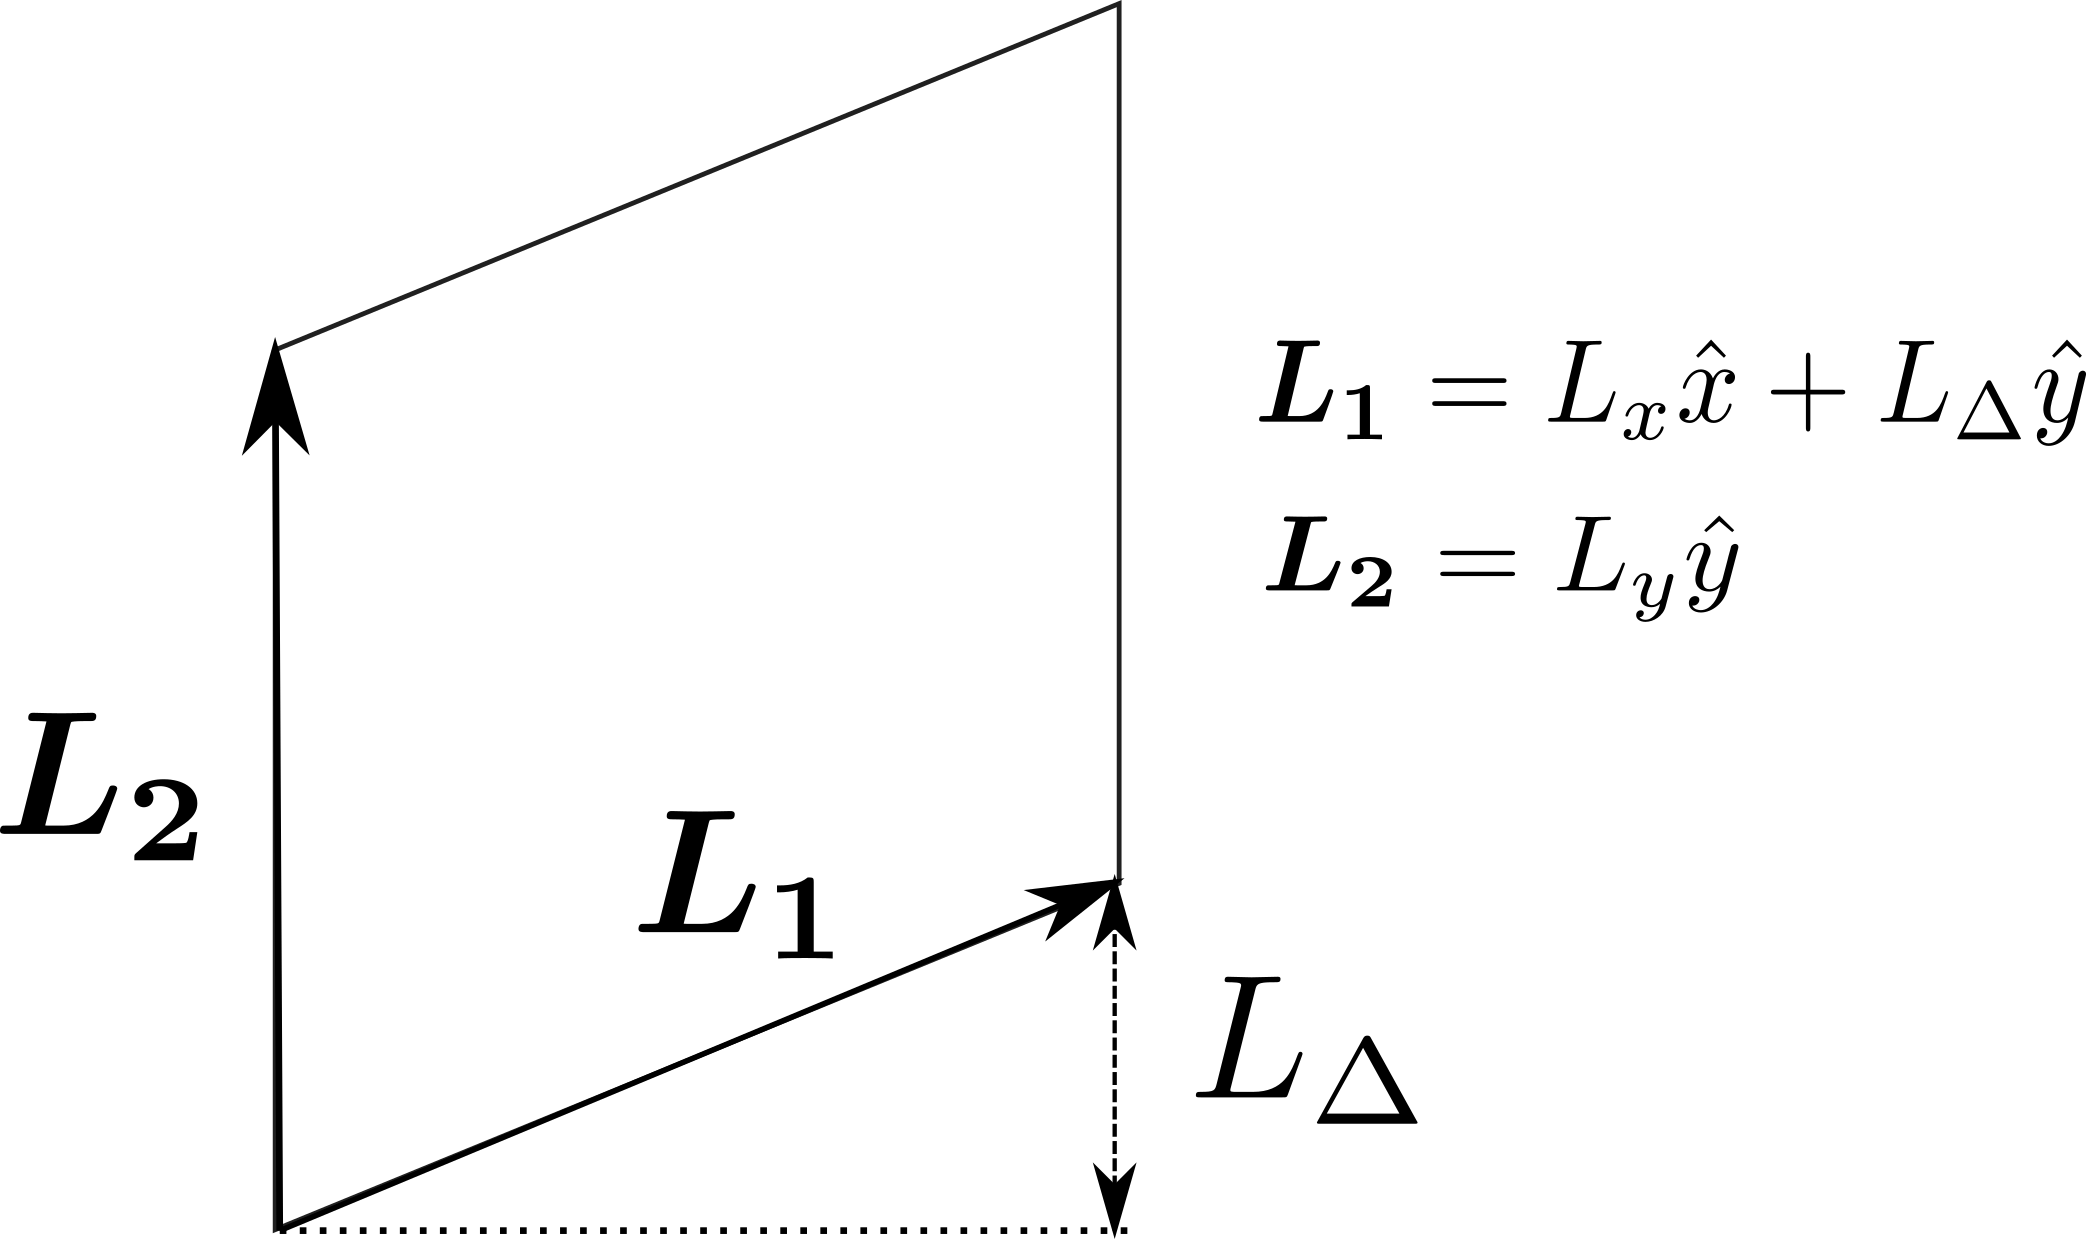
\includegraphics[width=2.5in]{figures/pngs/unit_cell_torus.png}
   			\caption{Unit cell}
    			\label{fig1}
  		\end{figure}

  		Then we demand that the physical observables of the system should not change if any particle(s) is(are) 
  		translated by a vector
  
  		\begin{equation*}
    			\bsym{L_{m,n}} = m\bsym{L_1} + n\bsym{L_2}\quad m,n \in  \mathbb{Z}
  		\end{equation*}
  
  			Because such translation brings back the particle in the same position because of imposed pbc. So this 
  			is the first symmetry we have on torus geometry and we will see its implications on a qhe system next.

	\subsection{Magnetic Translation Operator [MTO]}
  		In the absense of magnetic field, the generator of translation is canonical momenta. That is

  		\begin{align}
    			T(\vec{a}) &= \text{exp}\left( \frac{\iota}{\hbar}{\vec{a}\cdot\bsym{P}}\right) \\
    			\implies \quad T(\vec{a})\psi(\vec{x}) &= \psi(\vec{x}+\vec{a}) \non
  		\end{align}
  			  
  		The quantum Hall Hamiltonian looks like 

		\begin{equation}
			H = \sum_{i}\frac{{\bsym{\pi}_{i}}^{2}}{2m}  + \frac{1}{2}\sum_{i,j} V(\vec{r_i}-\vec{r_j})
		\end{equation}
		
		with $V(\vec{r}_{i,j} + \boldsymbol{L_{m,n}})=V(\vec{r}_{i,j})$ on torus, where $\bsym{\pi}$'s are the 
		physical momenta given as 
		
		\begin{equation*}
			\bsym{\pi} = \bsym{p} + |e|\bsym{A}(\bsym{r})
		\end{equation*}
		
		where $\bsym{A}(\bsym{r})$ is the magnetic potential and -ve charge of the electron is accounted for.\\
		
		The interest in translation operator, $T$, is as an accompanying symmetry of $H$ in torus, with a possible 
		reduction of H in smaller sectors corresponding to q-numbers of $T$. But here is a problem : even though, 
		we have canonical momentum commuting with each other
		
		\begin{equation*}
			[p_x,p_y] = 0
		\end{equation*}
		
		But physical moments do not commute
		
		\begin{equation*}
			[\pi_x,\pi_y] \neq 0
		\end{equation*}
		Implying, $[H,\bsym{p}]\neq 0$. Thus translations generated with $\bsym{p}$ or $\bsym{\pi}$ will not 
		commute with $H$.
		
		There is a way to remove the non-commuting part from the $\bsym{\pi}$ operators as follows
		
		\begin{align}
			\bsym{K} &= \bsym{\pi} - \frac{\hbar}{l^2}(\hat{z}\times \bsym{r}) \\
			\text{or}\quad \bsym{K} &= \bsym{\pi} - eB(\hat{z}\times \bsym{r}) \non
		\end{align}
		
		such that 
		
		\begin{align*}
			[\bsym{K},\bsym{\pi}]&=0 \\
			\implies\quad [\bsym{K},H]&=0 
		\end{align*}
				
			
		If we make a modified ``translation" operator using $\bsym{K}$, as follows
		
		\begin{align}
    			T(\vec{a}) &= \text{exp}\left( \frac{\iota}{\hbar}{\vec{a}\cdot\bsym{K}}\right)
    		\end{align}
		 
		which commutes with $H$, how do we know its action brings the right translation? Else why we are calling 
		it a translation operator at all?\\

		Let's go back to the form of $\bsym{K}$ to check this
		
		\begin{align*}
    			\bsym{K} &= \bsym{p} + e\bsym{A}(\bsym{r}) - eB(\hat{z} \times \bsym{r}) \\
    			\text{say}\quad \bsym{R} &= e\bsym{A}(\bsym{r}) - eB(\hat{z} \times \bsym{r})
    		\end{align*}
		
		Using $e^{A+B} = e^{A}e^{B}e^{-\frac{1}{2}[A,B]}$, where $[A,B]$ is c-number, we can find that
		
		\begin{align}
    			\nexp{\frac{\niota}{\hbar}\bsym{a} \cdot \bsym{K}}  &=  \nexp{\frac{\niota}{\hbar}\bsym{a} \cdot \bsym{p}} \nexp{\frac{\niota}{\hbar}\bsym{a}\cdot\bsym{R}}\nexp{\frac{1}{2\hbar^{2}}[\bsym{a}\cdot\bsym{p},\bsym{a}\cdot\bsym{R}]}
    		\end{align}
		
		let's call $\nexp{\frac{\niota}{\hbar}\bsym{a} \cdot \bsym{p}}$, the normal translation operator $T_{\bsym{p}}\cbrak{\bsym{a}}$. Then

		\begin{align}
    			[\bsym{a}\cdot\bsym{p},\bsym{a}\cdot\bsym{R}] &= [p_{x}a_{x}+ p_{y}a_{y},e(a_{x}A_{x}(\bsym{r})+a_{y}A_{y}(\bsym{r}))-eB(-a_{x}y+a_{y}x)] \\
    			&= e{a_{x}}^{2}[p_{x},A_{x}(\bsym{r})] + e{a_{x}a_{y}}[p_{x},A_{y}(\bsym{r})] + e{a_{y}}^{2}[p_{y},A_{y}(\bsym{r})] + \non \\ 
    			&\quad e{a_{x}a_{y}}[p_{y},A_{x}(\bsym{r})]-eBa_{x}a_{y}[p_{x},x] + eBa_{x}a_{y}[p_{y},y] \non \\ 
    			&= e{a_{x}}^{2}[p_{x},A_{x}(\bsym{r})] + e{a_{x}a_{y}}[p_{x},A_{y}(\bsym{r})] + e
    			{a_{y}}^{2}[p_{y},A_{y}(\bsym{r})] + \non \\ 
    			&\quad e{a_{x}a_{y}}[p_{y},A_{x}(\bsym{r})] \non
    		\end{align}
    		
    		Assuming $\bsym{A}(\bsym{r})$ is linear in $\bsym{r}$, all the commutators will give c-number.  
    		
    		\begin{align}
    			\bsym{a}\cdot\bsym{R} &= e(a_{x}A_{x}(\bsym{r})+a_{y}A_{y}(\bsym{r}))-eB(-a_{x}y+a_{y}x)
    		\end{align}
    		
    		If we look at general $\bsym{A}(\bsym{r})$, it is hard to see action of $eB(\hat{z} \times \bsym{r})$ , but if we take Landau's gauge $\bsym{A}(\bsym{r}) = Bx\hat{y}$, using \req{6} and \req{7}. we have
    		
    		\begin{align*}
    			\nexp{\frac{\niota}{\hbar}\bsym{a} \cdot \bsym{K}} &= \tnorm{a} \nexp{\frac{\niota}{\hbar}(eBxa_{y}-eB(-a_{x}y+a_{y}x))} \nexp{\frac{1}{2\hbar^{2}}(eBa_{x}a_{y}(-\niota\hbar))} \\
    			&= \tnorm{a} \nexp{\frac{\niota}{\hbar}(eBa_{x}y)} \nexp{-\frac{\niota}{2l^{2}}(a_{x}a_{y})} \\
    			&= \tnorm{a} \nexp{\frac{\niota}{l^{2}}(a_{x}y-\frac{1}{2}a_{x}a_{y})}  \\
    			&=  \nexp{\frac{\niota}{l^{2}}(a_{x}(y+a_y)-\frac{1}{2}a_{x}a_{y})}\tnorm{a}  \\
    			\tmag{a} &=  \nexp{\frac{\niota}{l^{2}}(a_{x}y+\frac{1}{2}a_{x}a_{y})}\tnorm{a}  \\
    		\end{align*}
    		
    		Thus magnetic translation operator $\tmag{a}$ does something more than the normal translation $\tnorm{a}$. It compensates for any changes in $\psi(\bsym{r})$ because of $\bsym{A}(\bsym{r})\rightarrow \bsym{A}(\bsym{r}+\bsym{a})$. Thus, the eigenstates of $H$, $\{\psi(\bsym{r})\}$, on torus, will follow
    		
    		\begin{align*}
    			\tmag{\bsym{L_{m,n}}}\psi(\bsym{r}) = \psi(\bsym{r})\\
    			\text{but not}\quad \tnorm{\bsym{L_{m,n}}}\psi(\bsym{r}) = \psi(\bsym{r})
    		\end{align*}
    		
    		\section{MTO Algebra}
                \hrulefill
                
    		\subsection{Single Particle Translations}
    		
    		From now on, all translations will automatically mean magnetic, unless mentioned otherwise. First of all, the sum of two tranlations
		
		\begin{align*}
			\tmag{\bsym{a}+\bsym{b}} &= \tmag{\bsym{a}}\tmag{\bsym{b}}\nexp{\frac{1}{2\hbar^{2}}[\bsym{a}\cdot\bsym{K},\bsym{b}\cdot\bsym{K}]} \\
			[\bsym{a}\cdot\bsym{K},\bsym{b}\cdot\bsym{K}] &=  [a_{x}p_{x}+a_{y}p_{y}-eB(-a_{x}y+a_{y}x),b_{x}p_{x}+b_{y}p_{y}-eB(-bs_{x}y+b_{y}x)] \\
			&= eB[a_{x}p_{x}+a_{y}p_{y},b_{x}y-b_{y}x] + eB[a_{x}y-a_{y}x,b_{x}p_{x}+b_{y}p_{y}] \\
			&= eBa_{x}b_{y}(\niota\hbar) - eBa_{y}b_{x}(\niota\hbar) + eBa_{x}b_{y}(\niota\hbar)  - eBa_{y}b_{x}(\niota\hbar) \\
			&=  2\niota\hbar eB(\bsym{a}\times\bsym{b})\cdot \hat{z}
		\end{align*}
		
		\begin{tcolorbox}[ams align]
			\implies\quad \tmag{\bsym{a}+\bsym{b}} &= \tmag{\bsym{a}}\tmag{\bsym{b}}\nexp{\frac{\niota}{l^{2}}(\bsym{a}\times\bsym{b})\cdot \hat{z}} \\
			\implies\quad [\tmag{\bsym{a}},\tmag{\bsym{b}}] &= -2\niota\ \nsin{\frac{1}{l^{2}}(\bsym{a}\times\bsym{b})\cdot \hat{z}} \tmag{\bsym{a}+\bsym{b}}
		\end{tcolorbox}		

	    We know that in a planar geometry, the degeneracy of each Landau level (LL) is equal to the number of flux quantas $(\phi_{\circ}=h/e)$ passing through the total area of sample which is given as $\hat{z}\cdot({\bsym{L_1}\times \bsym{L_2}})$
	    \begin{equation*}
	    		N_{\phi}  = \hat{z}\cdot({\bsym{L_1}\times \bsym{L_2}})/{2\pi l^{2}}
	    \end{equation*}
	    
	    From now on, we take magnetic length $l=1$. Then $2\pi N_{\phi} = \hat{z}\cdot({\bsym{L_1}\times \bsym{L_2}})$. \textcolor{red}{(Why the number of flux quanta has to be an integer?)}.\\
  
	    Anyway, for qhe, $\np$ is an integer, hence \req{8} and \req{9} tell us that
	    
	    \begin{align*}
		    \tmag{L_1+L_2} &= \tmag{L_1}\tmag{L_2} \\
		    \tmag{mL_1+nL_2} &= \tmag{mL_1}\tmag{nL_2} \\
	  		[\tmag{mL_{1}},\tmag{nL_{2}}] &= 0
	    \end{align*}
	    
	    We want to have simultaneous eigenfunctions for $H$ and $\tmag{L_{m,n}}$ such that
	    \begin{tcolorbox}[ams equation]
	    		\ti{i}{L_{m,n}}\psi(\bsym{r})  = \psi(\bsym{r}+\bsym{L_{m,n}})= \nexp{\niota \theta^{i}_{m,n}}\psi(\bsym{r})
	    \end{tcolorbox}
	    
		But since we are dealing with identical particles, exchanging 2 particles results in getting an overall sign to wavefunction. Implies that
		
		\begin{align*}
                  \ti{i}{L_{m,n}} \Psi(..,r_i,..,r_j,..) &= -\ti{i}{L_{m,n}}(i\leftrightarrow j) \Psi(..,r_i,..,r_j,..) \\
                                                         &= -\ti{i}{L_{m,n}} \Psi(..,r_j,..,r_i,..)\\
                                                         &= -\Psi(..,r_j+L_{m,n},..,r_i,..)\\
                  \implies\quad \nexp{\niota \theta^{i}_{m,n}} &= \nexp{\niota \theta^{j}_{m,n}}
                \end{align*}
                
                hence, the eigenvalue should not depend on the particle index. Which means $\theta^{i}_{m,n}=\theta^{j}_{m,n}=\theta_{m,n}$.
                So if we have
                
                \begin{align*}
                  \ti{i}{mL_{1}+nL_{2}} &= \ti{i}{mL_{1}}\ti{i}{nL_{2}}\nexp{\frac{\niota}{2l^2}\hat{z}\cdot(\bsym{L_1}\times\bsym{L_2})}  \\
                                        &= {\ti{i}{L_{1}}}^{m}{\ti{i}{L_{2}}}^{n}\nexp{\niota \pi N_{\phi} mn}
                \end{align*}

                \begin{tcolorbox}[ams equation]
                  \implies\quad \theta_{m,n} = \pi mn N_{\phi} + m\theta_{1} +n\theta_{2}
                \end{tcolorbox}

                \subsection{Many Particle Translations}

                Now we move to two types of collective translations :

                \begin{enumerate}
                \item  $\tcm{a}$ center of mass translations 
                \item $\trel{i}{a}$ relative translations  
                \end{enumerate}

                Action of $\tcm{a}$ is pretty straightforward as all the particles are translated via same vector $\bsym{a}$. The Hamiltonian doesn't care about CoM translation as all the relative distances remain the same. Hence $[H,\tcm{a}]=0$.

                \pagebreak

                \begin{figure}[h]
                  \centering
                  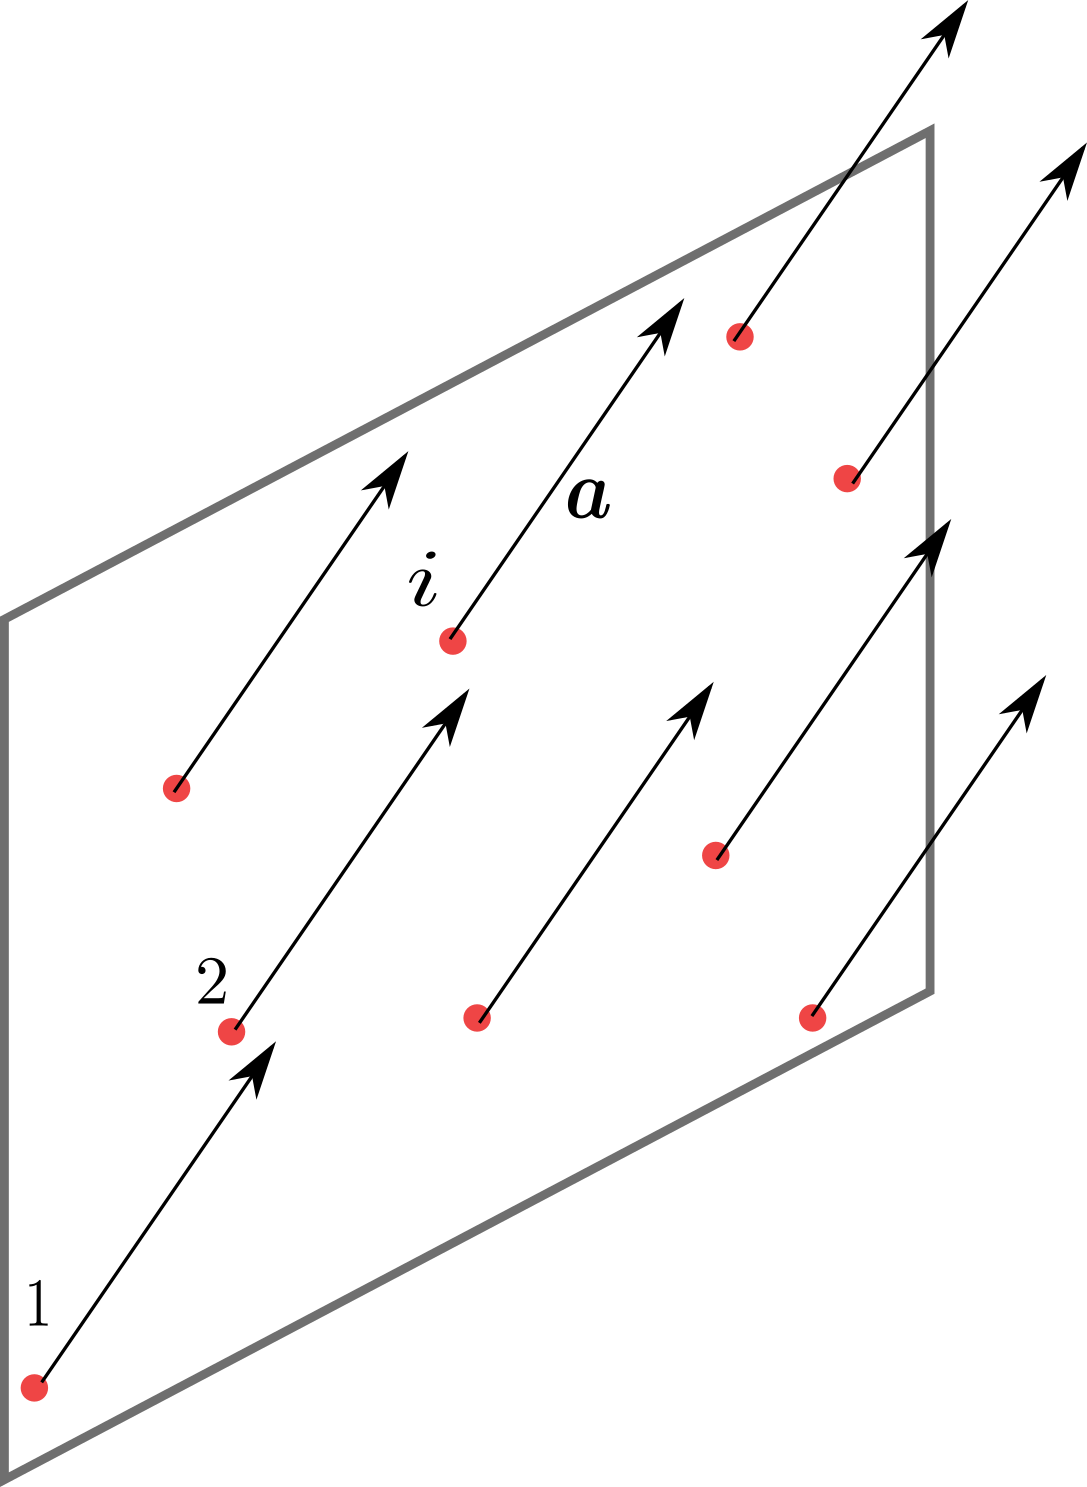
\includegraphics[width=2in]{figures/pngs/t_cm.png}
                  \hspace{1cm}
                  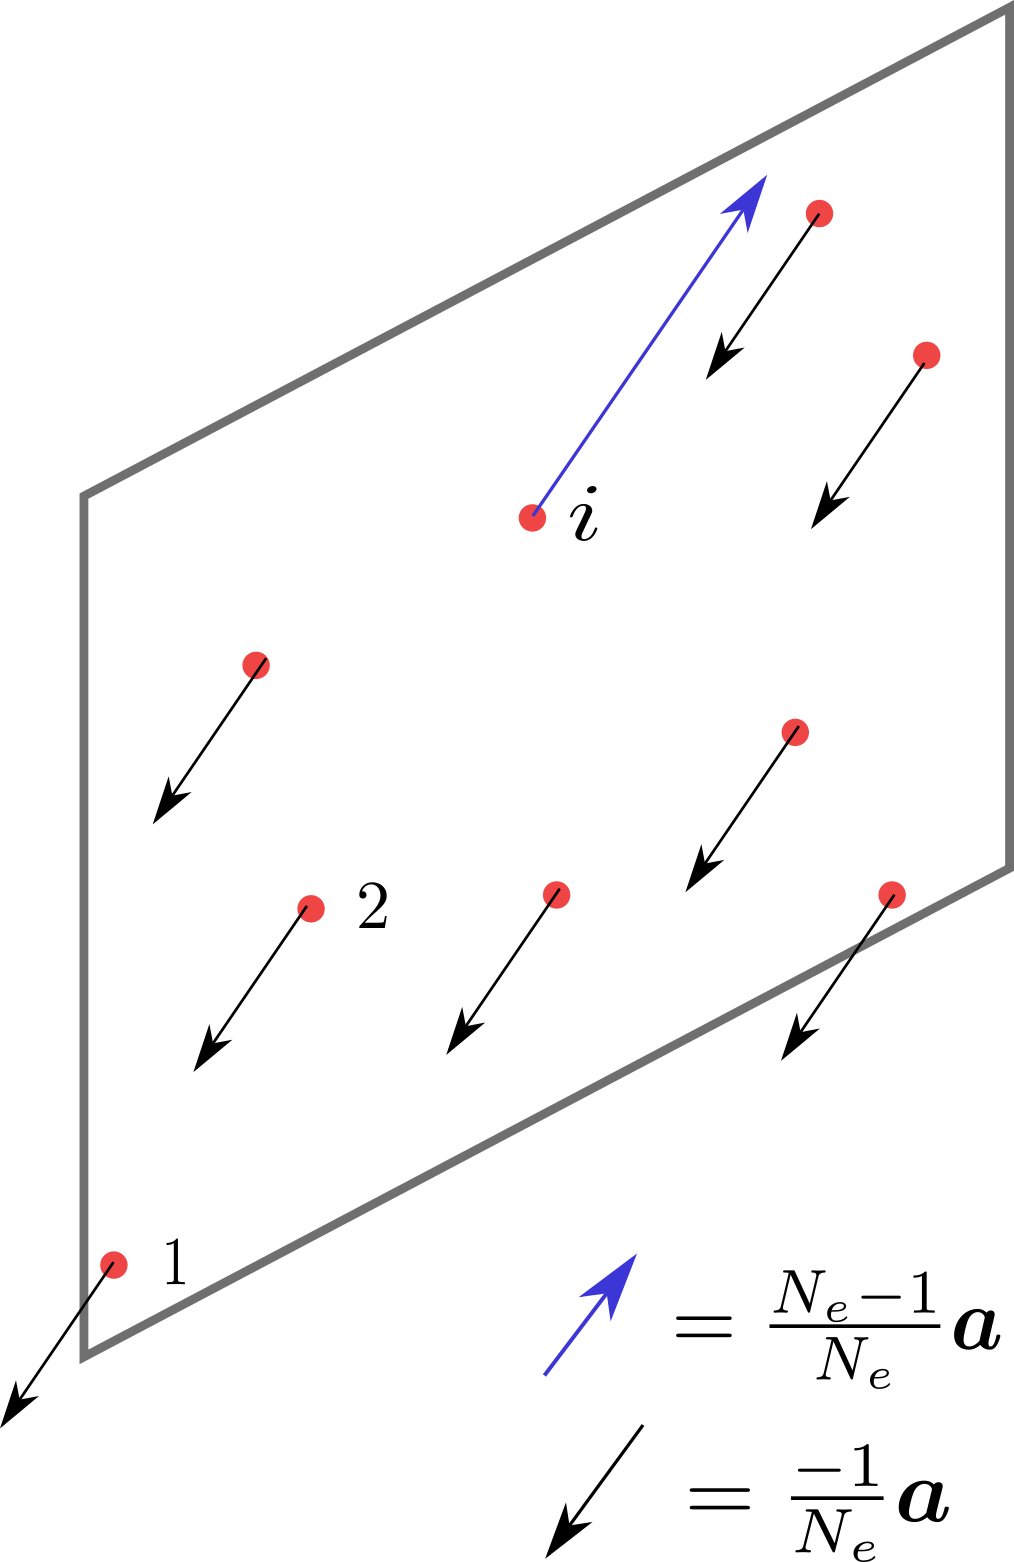
\includegraphics[width=2in]{figures/pngs/t_rel.png}
                  \caption{Action of $\tcm{a}$ and $\trel{i}{a}$}
                \end{figure}

                In the case of relative translation, $\trel{i}{a}$, one achieves translation of $i^{th}$-particle by $\bsym{a}$ by moving it by $\frac{N_{e}-1}{N_{e}}\bsym{a}$ and all the other particles in the opposite direction by $\frac{-\bsym{a}}{N_{e}}$ where $N_{e}$ is the number of particles.\\

                But even though, $\tcm{a}$ commutes with $H$, but it doesn't commute with $\ti{i}{a}$ for all $\bsym{a}$. So if we would want to find out the translations for which they commute. Since $\ti{i}{a}$'s commute for different $i$'s, all we have to check is

                \begin{equation*}
                  [\ti{i}{a},\ti{i}{L_{m,n}}] = 0
                \end{equation*}

                where \req{9} tells us, for $\bsym{a} = \alpha \hat{x} + \beta \hat{y} $,
                \begin{align*}
                  \frac{1}{l^2}(\bsym{a}\times \bsym{L_{m,n}})\cdot\hat{z} &= \frac{1}{l^2} (-m\beta L_{x} + m\alpha L_{\Delta}+n\alpha L_{y}) = k\pi\quad k\in\mathbb{Z}
                \end{align*}

                Since this should for work for many $m,n$, say we have $m=0$, then

                \begin{align*}
                  \frac{\alpha L_{y}}{2l^{2}} &= k_{1}\pi\quad k_{1}\in\mathbb{Z} \\
                  \alpha &= k_{1}\frac{L_{x}}{\np}
                \end{align*}

                and for $n=0$, we will have

                \begin{align*}
                  \frac{\alpha L_{\Delta} - \beta L_{x}}{2l^2} &= k_{2}\pi\quad K_{2}\in\mathbb{Z} \\
                  \text{putting in the value of }\alpha & \\
                  \frac{L_{x}}{2l^{2}}(-\beta + \frac{k_1}{\np}L_{\Delta}) &= k_2\pi \\
                  \cbrak{k_{1}\frac{L_{\Delta}}{L_{y}}-\beta\frac{\np}{L_{y}}} &= k_{2} \\
                  \beta & = \cbrak{k_{1}\frac{L_{\Delta}}{\np} - k_2\frac{L_y}{\np}}
                \end{align*}

                Putting in the values of $\alpha$ and $\beta$, we have

                \begin{align}
                  \bsym{a} &=\cbrak{k_{1}L_{x}\hat{x} + (k_1L_{\Delta}+k_2L_{y})\hat{y}}/\np \non \\
                  & = \bsym{L_{k_1,k_2}}/\np \non
                \end{align}

                Hence all the CoM of translations of such form don't change the representation of $\ti{i}{a}$'s

                \begin{tcolorbox}[ams equation]
                  \implies [\tcmnp{L_{m,n}},\ti{i}{L_{k,l}}] = 0\quad m,n,k,l\in\mathbb{Z}
                \end{tcolorbox}

                But remember, we would also want there CoM translations to commute with each others too. We'll come to this point later.\\

                In case of relative translations, $\trel{i}{a}$ (which commutes with any $\tcm{b}$) we need following conditions to satisfy :

                \begin{enumerate}
                \item $[\trel{i}{a},\ti{i}{L_{m,n}}]  = 0$
                \item $[\trel{i}{a},\ti{j}{L_{m,n}}]  = 0$
                \item $[\trel{i}{a},\trel{i}{b}]  = 0$
                \item $[\trel{i}{a},\trel{i}{b}]  = 0$
                \end{enumerate}

                Now, we consider such systems where $N_{e}=pN$ and $\np = qN$ such that $\text{gcd}(p,q)=1$. Under such assumptions, only $\bsym{a} = p\bsym{L_{m,n}}$
                satisfies all four conditions. \textcolor{red}{(Add the proof later!)}

                So far, we have

                 \begin{itemize}
                 \item $\ti{i}{L_{m,n}}$, single particle translation, which commutes with $H$ and assigns each eigenstates with an eigenvalue $\nexp{\niota \theta_{m,n}}$. As shown in \req{11}, this depends upon what we chose as the eigenvalues of translations corresponding to $\bsym{L_1}$ and $\bsym{L_{2}}$. This choice defines the representation of these and many-body translation operators as well.
                 \item $\tcmnp{L_{m,n}}$, CoM translation, which commute with $H$ and $\trel{i}{a}$ for any translation $\bsym{b}$. But to commute with any $\ti{i}{L_{k,l}}$, we need $\bsym{b}=\bsym{L_{m,n}/np}$. But even after assuring all the necessary commutations, we can't guarantee the commutations between different CoM translations. That will be discussed later.
                 \item $\trel{i}{pL_{m,n}}$, relative translation, which commutes with all $H$, $\ti{i}{L_{i,j}}$ and $\trel{i}{pL_{k,l}}$. 
                 \end{itemize}

                 \section{Building the Hilbert Space}
                 \hrulefill

                 We have the single particle wavefunction for the case of $V(\bsym{r})=0$, which is a slight modification of Iqhe wf, to account for the periodicity of torus.
                 \begin{tcolorbox}[ams align]
                   \phi_{m,j}(x,y) &= \sum_{k} \nexp{\frac{\niota}{2}\cbrak{j\frac{L_{x}}{\np}+kL_{x}}\cbrak{j\frac{L_{\Delta}}{\np}+kL_{\Delta}}} \non \\
                   & \times \nexp{-\frac{2\pi \niota}{L_{y}}\cbrak{j+k\np}} \sqexp{ -\frac{1}{2} \nbrak{ \frac{x}{l} - \frac{2\pi l}{L_y} (j+k\np) }^{2} } \non \\
                   & \times H_m \left[ \frac{2\pi l}{L_y} (j+k\np) -\frac{x}{l} \right]
                 \end{tcolorbox}
              \end{document}